% ================================================================
%  TokenMizer: Graph-Structured Session Memory for
%  Long-Horizon LLM Context Management
%  IEEE Transactions Style — Journal Version
%
%  Single-version manuscript. Evaluates TokenMizer 0.5.4 (the
%  released product, https://github.com/Shweta-Mishra-ai/tokenmizer)
%  against seven other memory methods on a 100-session labelled
%  corpus. All values in this manuscript are measured against the
%  corpus and code released at
%  https://github.com/Shweta-Mishra-ai/tokenmizer-research.
%  No estimated results are presented.
% ================================================================
\documentclass[journal]{IEEEtran}

\usepackage{amsmath,amssymb,amsthm}
\usepackage{graphicx}
\usepackage{booktabs}
\usepackage{array}
\usepackage{colortbl}
\usepackage{xcolor}
\usepackage{url}
\usepackage{balance}
\usepackage{multirow}
\usepackage{algorithm}
\usepackage{algorithmic}
\usepackage[colorlinks=true,
            linkcolor=blue!60!black,
            citecolor=blue!60!black,
            urlcolor=blue!60!black]{hyperref}

\definecolor{rowours}{HTML}{FEF9C3}
\definecolor{rowgood}{HTML}{DCFCE7}
\definecolor{rowwarn}{HTML}{FEE2E2}

\newtheorem{definition}{Definition}
\newtheorem{proposition}{Proposition}

\tolerance=9999
\emergencystretch=4em
\hbadness=10000

% ================================================================
\title{TokenMizer: Graph-Structured Session Memory\\
for Long-Horizon LLM Context Management}

\author{Shweta~Mishra%
\thanks{Independent Researcher, India.
E-mail: \href{mailto:shweta.mishra.research@gmail.com}{shweta.mishra.research@gmail.com}.
Product: \url{https://github.com/Shweta-Mishra-ai/tokenmizer} (evaluated
at release 0.5.4).
Benchmark suite, corpus, and reproduction code for this manuscript:
\url{https://github.com/Shweta-Mishra-ai/tokenmizer-research}.
Manuscript received June 4, 2026; revised August 13, 2026.}%
}

% ================================================================
\begin{document}
\maketitle

% ================================================================
\begin{abstract}
Large language model (LLM) deployments for long-horizon tasks
face a fundamental constraint: context windows are finite while
productive work sessions are not.
When session history exceeds the Maximum Effective Context
Window (MECW), critical structured information---architectural
decisions, task status transitions, file modification histories,
and resolved errors---is silently discarded.
Existing mitigations (truncation, summarization, retrieval
augmentation) treat history as flat text, destroying the typed,
relational structure that makes sessions resumable.

We present \textbf{TokenMizer}, an open-source proxy system
that models LLM session history as a typed knowledge graph
(14 node types, 8 edge types) populated by a hybrid extraction
pipeline, serialized by a three-tier checkpoint system into
compact resume blocks, and supported by an 8-layer compression
pipeline and a semantic response cache.

We evaluate TokenMizer 0.5.4 --- the released product, run
unmodified and out-of-process against a real checkout --- on a
controlled \textbf{100-session, 8-method} benchmark: 100 labelled
sessions (94 constructed for this study, 6 real, spanning 23
application domains) scored against TokenMizer and seven other
memory methods under one shared, asymmetric coverage-based
scorer, with \textbf{bootstrap 95\% confidence intervals}
(3{,}000 resamples) on every reported comparison.
Four of the seven comparison methods are deterministic
reimplementations of one structural property each of MemGPT,
Mem0, Graphiti/Zep, and GraphRAG, run with no language-model
call; this is a methodologically load-bearing distinction we
state precisely in Section~\ref{sec:threats} and repeat at
every point the comparison is reported.

TokenMizer scores $60\%$ macro F1 ($95\%$ CI $[55\%,65\%]$),
significantly higher than the GraphRAG-style ($44\%$),
MemGPT-style ($35\%$), and all three naive baselines
($17$--$20\%$) reimplementations, and \emph{statistically
indistinguishable} from the Graphiti-style ($59\%$) and
Mem0-style ($60\%$) reimplementations (paired bootstrap $95\%$
CI on the difference crosses zero for both; TokenMizer's point
estimate matches Mem0-style's exactly).
TokenMizer's resume block (100 tokens) is smaller than
Graphiti-style's and Mem0-style's (118--120) but larger than
MemGPT-style's (60), which reaches that size by seeing under
half the conversation rather than by encoding it more
efficiently.
Its two weakest categories, both in absolute terms and relative
to the two comparison methods it otherwise ties, are decision
extraction ($59\%$ F1, against $65\%$ for Graphiti/Mem0-style)
and error extraction ($44\%$ F1, against $66\%$).
Every pattern-matching method tested, TokenMizer included,
degrades to $19$--$27\%$ macro F1 on sessions that state facts
indirectly rather than with explicit lexical markers---a
shared ceiling of regex-based extraction that this study is,
to our knowledge, the first to quantify across multiple
independently-implemented memory strategies on one corpus.

TokenMizer is released as open-source software (MIT licence).
The 100-session corpus, all eight method implementations, the
scoring harness, and raw per-session results are released
alongside this manuscript for independent verification.
\end{abstract}

\begin{IEEEkeywords}
large language models, context management, session memory,
knowledge graph, prompt compression, semantic caching,
long-horizon tasks, benchmark evaluation, information extraction
\end{IEEEkeywords}

% ================================================================
\section{Introduction}
\label{sec:intro}
% ================================================================

\IEEEPARstart{L}{arge} language model (LLM) deployments for
software engineering~\cite{sweagent,copilot}, data
science~\cite{housurvey}, and research assistance increasingly
involve \emph{long-horizon sessions}: multi-turn interactions
spanning hours, where each turn builds on the accumulated
context of previous turns.
These sessions develop rich internal structure: technology
choices made in turn 3 constrain implementation options in
turn 12; errors resolved in turn 7 inform test strategies in
turn 15; files modified in turn 4 must be updated consistently
in turn 18.

The fundamental constraint is context window capacity.
Paulsen~\cite{paulsen2025} defines the \emph{Maximum Effective
Context Window} (MECW) as the context length at which model
task accuracy degrades below an acceptable threshold.
Critically, MECW is substantially lower than the advertised
maximum context window (MCW) for complex, multi-step tasks.
Liu et al.~\cite{lostmiddle} further demonstrate that content
placed in the \emph{middle} of long contexts is systematically
under-attended, amplifying the effective degradation.
At approximately 950~tokens per turn, a development session
exhausts a 16{,}000-token MECW after only 16~turns.

\subsection{Limitations of Existing Approaches}

Three categories of mitigation exist, each with a structural
limitation.

\textbf{Truncation-based methods}~\cite{brownfewshot} discard
the oldest messages when the context budget fills.
This preserves recency but discards exactly the content
that matters most: architectural decisions, initial technology
choices, and goal definitions established early in a session.

\textbf{Summarization-based methods}~\cite{langchain}
produce free-text summaries via a secondary LLM call.
These compress well but are structurally imprecise: a natural
language summary cannot reliably distinguish a \emph{completed}
task from a \emph{pending} one, nor can it preserve the
\emph{rationale} for a technology decision.

\textbf{Retrieval- and memory-augmented methods}~\cite{rag,memgpt,mem0,zep}
retrieve or store relevant facts on demand.
As Section~\ref{sec:related} details, these systems differ
substantially in whether retained facts are typed, whether
superseded facts are deleted or retained, and whether older
turns remain reachable without an explicit query --- design
choices this paper measures directly rather than assumes.

\subsection{Key Insight and Contributions}

The core insight motivating TokenMizer is that
\textbf{session history is not flat text---it is a structured
knowledge artifact}, containing tasks with status lifecycles,
decisions with rationales, files with modification histories,
resolved errors, and environment facts that scope all other
entities, connected by typed relationships
(\textsc{implements}, \textsc{fixes}, \textsc{depends-on}, etc.)
that encode causal and structural dependencies.
A representation that preserves this structure enables
efficient, queryable context preservation: discard the raw
conversation tokens, retain the typed graph, serialize to a
compact resume block.

\textbf{Contributions:}
\begin{enumerate}
\item A \textbf{formal typed knowledge graph schema} for LLM
  sessions with 14 node types, 8 edge types, and a well-defined
  status transition system (Section~\ref{sec:graph}).
\item A \textbf{hybrid extraction pipeline}, a
  \textbf{three-tier checkpoint system}, an \textbf{8-layer
  compression pipeline}, and a \textbf{semantic response cache}
  (Sections~\ref{sec:extraction}--\ref{sec:cache}).
\item A \textbf{controlled 100-session, 8-method comparison}
  against deterministic reimplementations of four published
  memory strategies (MemGPT, Mem0, Graphiti/Zep, GraphRAG) and
  three naive baselines, with bootstrap confidence intervals on
  every comparison, a register-stratified analysis isolating
  pattern-matching's central failure mode, and a released
  corpus, harness, and raw results for independent reproduction
  (Section~\ref{sec:extended}).
\end{enumerate}

% ================================================================
\section{Background and Related Work}
\label{sec:related}
% ================================================================

\subsection{Context Window Degradation}

Paulsen~\cite{paulsen2025} introduces the MECW concept,
demonstrating empirically that all tested frontier models
degrade in accuracy on multi-step tasks before reaching
their advertised MCW.
For a model with MCW\,=\,128{,}000 tokens, the MECW may be
as low as 16{,}000 tokens for complex coding tasks.
This motivates the 16k-token MECW used as the running example
throughout this paper.
Liu et al.~\cite{lostmiddle} demonstrate the ``lost in the
middle'' phenomenon: retrieval and multi-document QA tasks
show U-shaped accuracy profiles, with content in the middle
of long prompts systematically under-used.

\subsection{Memory Systems for LLMs}
\label{sec:related-memory}

\textbf{MemGPT}~\cite{memgpt} proposes an OS-inspired
hierarchical memory model distinguishing main context (fast,
limited) from external storage (slow, unlimited), with
paging between them driven by explicit function calls the
LLM itself issues.
Facts that page out of main context are not deleted, but they
are also not spontaneously recalled: reaching them again
requires the model to issue a targeted archival-search call.
Section~\ref{sec:memgpt-style} reimplements this core/archival
asymmetry deterministically and measures its consequence:
recall on facts stated early in a long session degrades once
they age out of the always-visible window.

\textbf{Mem0}~\cite{mem0} extracts short natural-language
memories from a conversation and stores them in a flat,
undifferentiated pool, using an LLM to decide, memory by
memory, whether a new fact adds, updates, or deletes an
existing one.
It has no typed schema and no explicit edge structure.

\textbf{Graphiti}~\cite{zep}, the temporal knowledge-graph
engine underlying Zep, represents facts as edges in a
bi-temporal graph: every edge carries a \texttt{valid\_at} and
an \texttt{invalid\_at} timestamp, and a superseded fact is
marked invalid rather than deleted.
This directly targets a failure mode TokenMizer's own
\textsc{supersedes} edge type (Table~\ref{tab:edgetypes}) was
designed for, making Graphiti the closest architectural
relative among the systems compared in
Section~\ref{sec:extended} and the one against which
TokenMizer's advantage is smallest.

\textbf{GraphRAG}~\cite{graphrag} builds knowledge graphs from
document corpora to improve retrieval-augmented summarization
over static text collections.
Its schema is entity- and community-oriented and carries no
task-lifecycle concept; Section~\ref{sec:extended} finds this
distinction empirically, not just architecturally: the
GraphRAG-style reimplementation is competitive with TokenMizer
on decisions and files but far behind on completed- and
pending-task recall.

\textbf{LangChain Memory}~\cite{langchain} provides several
memory backends including ConversationKGMemory, architecturally
similar to TokenMizer but using an untyped, schema-free graph
with extraction and lifecycle management left to the
application developer.

\subsection{Prompt Compression}

\textbf{LLMLingua}~\cite{llmlingua} and
\textbf{LongLLMLingua}~\cite{longllmlingua} use small proxy
LLMs to compute per-token importance scores, removing
low-importance tokens at 2--6$\times$ compression ratios.
TokenMizer incorporates LLMLingua-2 as optional layers in its
compression pipeline, applied after heuristic preprocessing
has removed structurally trivial content and after code
segments have been excluded from ML compression entirely
(Section~\ref{sec:compression}).

\textbf{RECOMP}~\cite{recomp} applies selective summarization
for retrieval-augmented generation, retrieving only relevant
passages.
TokenMizer applies structural extraction rather than textual
retrieval: the resume block is generated from graph state, not
retrieved text, enabling typed queries that passage retrieval
cannot natively support.

\subsection{Positioning}

Table~\ref{tab:related} summarizes the qualitative differences
among the systems above.
Section~\ref{sec:extended} is, to our knowledge, the first
evaluation to score TokenMizer, MemGPT-style paging, Mem0-style
flat storage, Graphiti-style temporal retention, and
GraphRAG-style entity extraction against one shared corpus and
one shared scorer, rather than citing each system's own
self-reported numbers on its own benchmark.

\begin{table}[t]
  \centering
  \caption{Qualitative Comparison with Related Systems.
  ``Deletes superseded facts'' distinguishes MemGPT/Mem0-style
  last-write-wins behavior from Graphiti's and TokenMizer's
  explicit supersession tracking.}
  \label{tab:related}
  \renewcommand{\arraystretch}{1.3}
  \footnotesize
  \begin{tabular}{@{}p{1.9cm}p{1.55cm}p{1.5cm}p{1.15cm}@{}}
    \toprule
    \textbf{System} & \textbf{Struct.\ graph} &
    \textbf{Deletes superseded} &
    \textbf{Cross-session} \\
    \midrule
    Sliding window      & None      & n/a (no memory) & No \\
    LangChain KG Mem.   & Untyped   & No               & Yes \\
    MemGPT~\cite{memgpt} & Vector DB & No (pages out)   & Yes \\
    Mem0~\cite{mem0}     & None (flat) & Yes (LLM-judged) & Yes \\
    Graphiti/Zep~\cite{zep} & Bi-temporal & No (invalidated) & Yes \\
    GraphRAG~\cite{graphrag} & Entity/comm. & n/a (static) & No \\
    \rowcolor{rowours}
    \textbf{TokenMizer}
      & \textbf{Typed, 14-class} & \textbf{No (edge)}
      & \textbf{Partial} \\
    \bottomrule
  \end{tabular}
\end{table}

% ================================================================
\section{Problem Formulation}
\label{sec:problem}
% ================================================================

\begin{definition}[LLM Session]
A session $S = \langle m_1, m_2, \ldots, m_n \rangle$ is an
ordered sequence of messages, each with token count
$\tau(m_i) > 0$. The cumulative token count at turn $t$ is
$T(t) = \sum_{i=1}^{t} \tau(m_i)$.
\end{definition}

\begin{definition}[Context Overflow]
A session overflows at the first turn $n^*$ such that:
\begin{equation}
  T(n^*) > T_{\mathrm{MECW}}
  \label{eq:overflow}
\end{equation}
For $\bar{\tau} = 950$ tokens/turn and
$T_{\mathrm{MECW}} = 16{,}000$:
$n^* = \lfloor 16{,}000 / 950 \rfloor = 16$.
\end{definition}

\begin{definition}[Structured Resume Block]
A resume block $R$ is a compact text representation of the
session knowledge graph $G$, serialized to at most
$T_{\mathrm{budget}}$ tokens.
After a checkpoint at turn $n^* - 2$, the new context is:
\begin{equation}
  C' = R \;\cup\; \{m_{n^*-1}, m_{n^*}\}
  \label{eq:resume}
\end{equation}
satisfying $|C'| \leq T_{\mathrm{MECW}}$ by construction.
\end{definition}

\begin{definition}[Category Coverage Score]
\label{def:coverage}
For a ground-truth item $g$ and a candidate extraction $c$,
coverage is the fraction of $g$'s content words present in
$c$, or exact substring containment for items of at least 6
characters:
\begin{equation}
  \mathrm{covers}(c, g) =
    \left(\;|g| \geq 6 \wedge g \in c\;\right) \;\vee\;
    \frac{|W_g \cap W_c|}{|W_g|} \geq \theta
  \label{eq:coverage}
\end{equation}
with $\theta = 0.6$ throughout this paper and $W_x$ the
content-word set of $x$ (stopwords removed).
Coverage is deliberately asymmetric: the denominator is always
the ground-truth item's token set, so a method cannot inflate
recall by emitting one long label containing every keyword ---
that label would also fail precision, defined symmetrically
over the same relation (Section~\ref{sec:extended-scoring}).
\end{definition}

% ================================================================
\section{System Architecture}
\label{sec:system}
% ================================================================

\subsection{Deployment Model}
\label{sec:deploy}

Figure~\ref{fig:arch} shows the system architecture.
TokenMizer operates as a transparent HTTP reverse proxy
implementing the OpenAI Chat Completions API.
The client configures \texttt{base\_url} to the TokenMizer
server; no application code changes are required beyond this
endpoint substitution.
An optional \texttt{session\_id} parameter in the request body
activates the full pipeline; its absence produces a transparent
passthrough with zero overhead, making adoption incremental.

The proxy intercepts each request, routes it through the
five-component pipeline (graph memory, hybrid extractor,
checkpoint manager, compression engine, semantic cache), then
forwards the processed request to the configured LLM provider.

\begin{figure}[t]
  \centering
  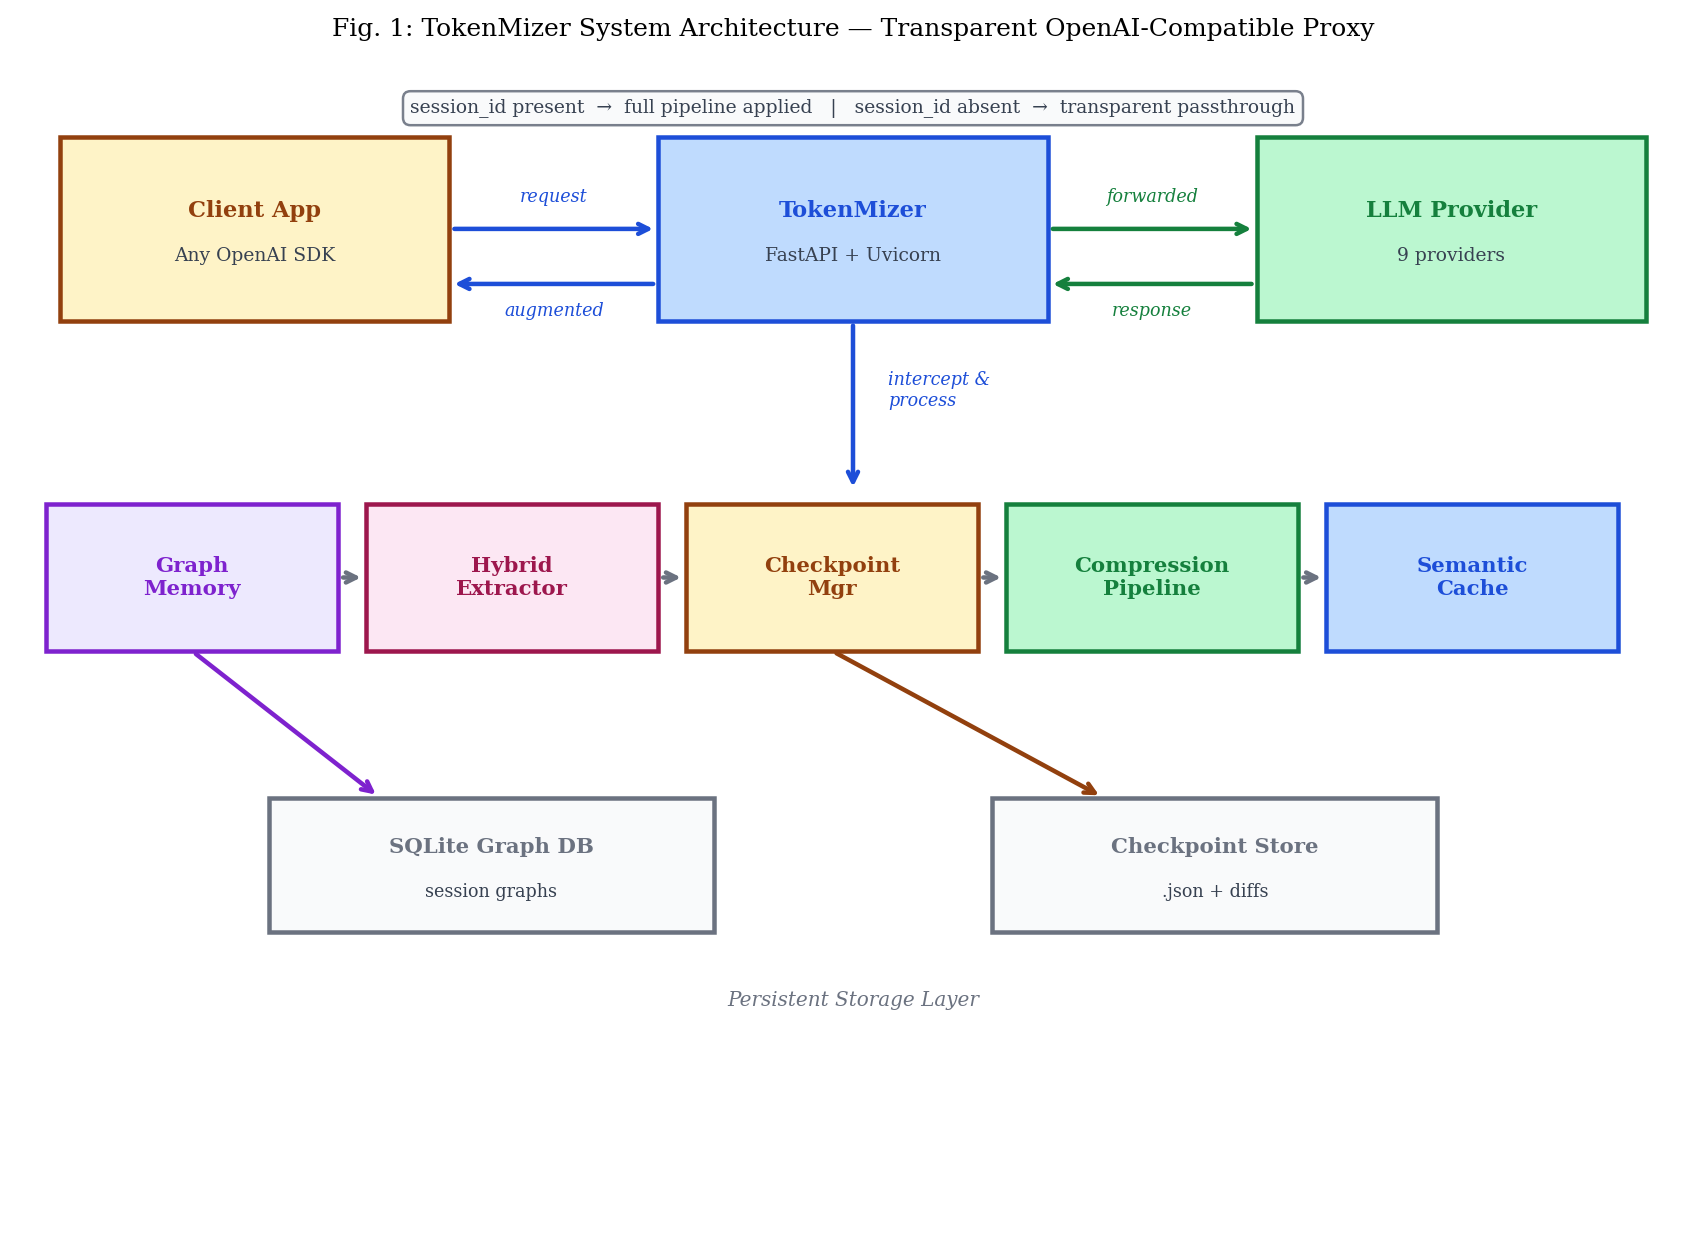
\includegraphics[width=\columnwidth]{fig1_architecture}
  \caption{TokenMizer system architecture. The proxy sits
    transparently between any OpenAI-compatible client and
    the LLM provider. When \texttt{session\_id} is present,
    the five-component pipeline is activated; otherwise the
    request passes through with no overhead. Persistent
    storage comprises a SQLite graph database and a JSON
    checkpoint store.}
  \label{fig:arch}
\end{figure}

\subsection{Knowledge Graph Schema}
\label{sec:graph}

Figure~\ref{fig:kgraph} illustrates a representative session
graph. The schema defines 14 node types across three
functional categories.

\begin{figure}[t]
  \centering
  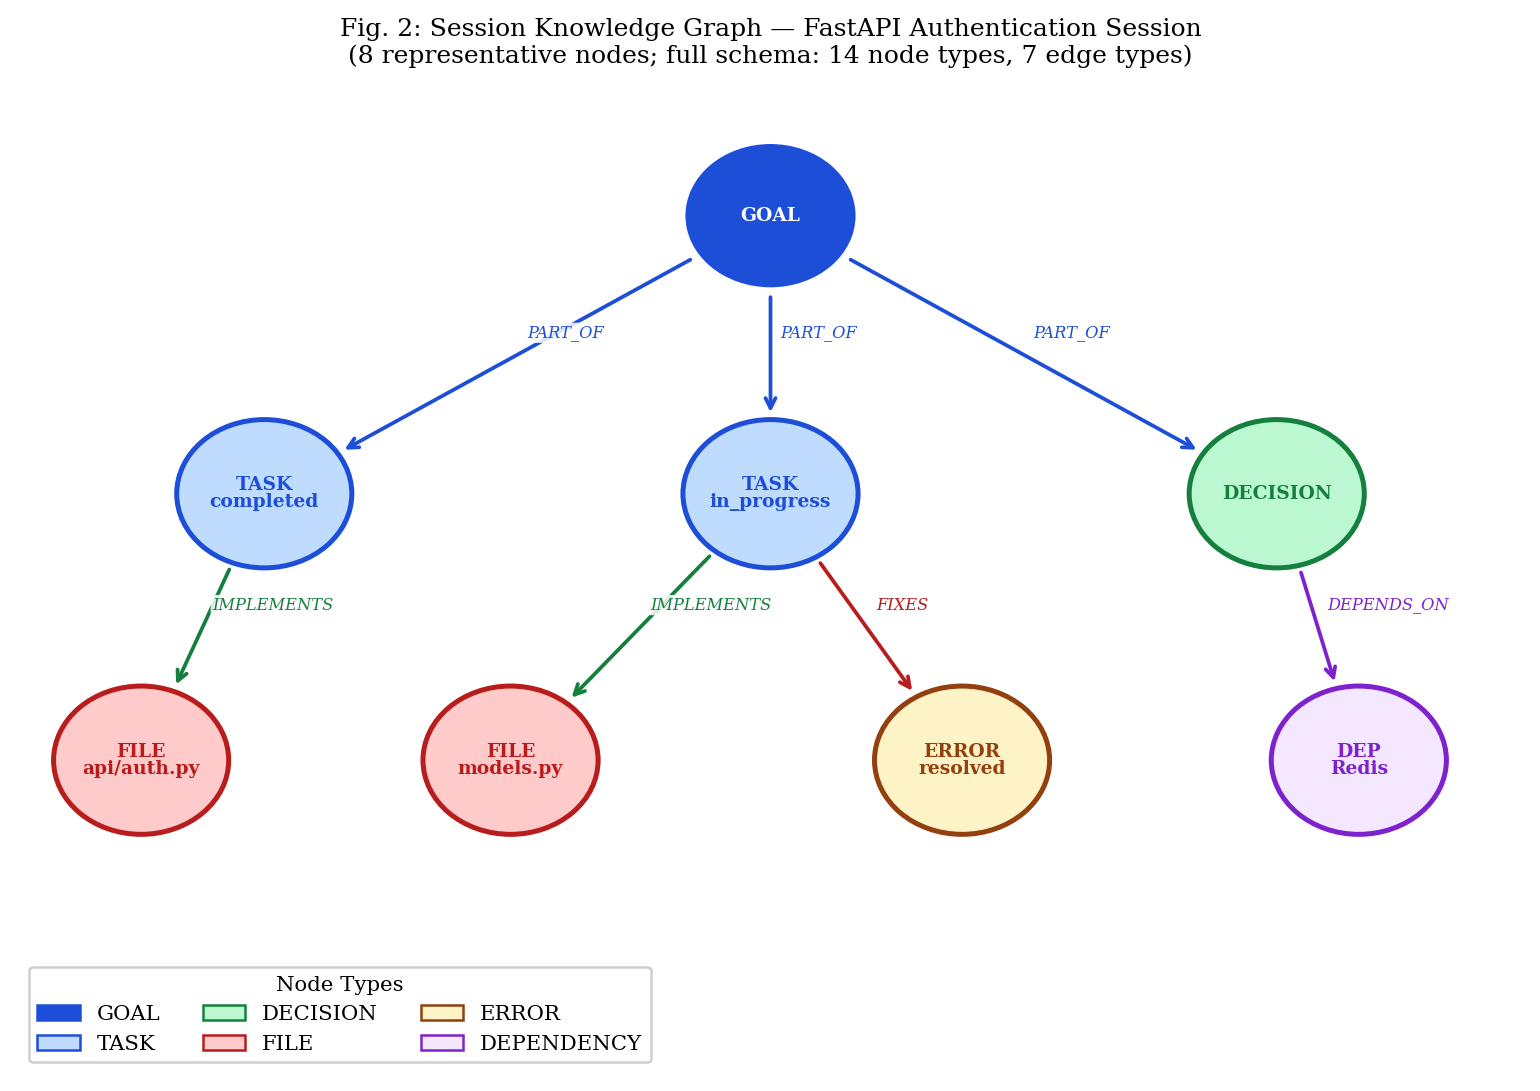
\includegraphics[width=\columnwidth]{fig2_graph}
  \caption{Session knowledge graph for a FastAPI
    authentication session (8 representative nodes).
    Edge labels show typed relationships; node colors
    indicate type. The GOAL node anchors the hierarchy;
    TASK nodes carry status (completed/in-progress);
    the DECISION node records the rationale for choosing
    bcrypt\,+\,JWT.}
  \label{fig:kgraph}
\end{figure}

\subsubsection{Node Types}
Table~\ref{tab:nodetypes} defines the 14 node types.
\emph{Action nodes} carry status lifecycles;
\emph{context nodes} are static.

\begin{table}[t]
  \centering
  \caption{Node Types (14 total). Action nodes carry status
  lifecycles (Pending, In-Progress, Completed, Failed,
  Contested). Context nodes are status-free.}
  \label{tab:nodetypes}
  \renewcommand{\arraystretch}{1.15}
  \begin{tabular}{@{}p{2.4cm}p{1.7cm}p{3.5cm}@{}}
    \toprule
    \textbf{Type} & \textbf{Category} & \textbf{Primary trigger} \\
    \midrule
    \texttt{TASK}       & Action    & Imperative verb + object \\
    \texttt{FILE}       & Action    & Extension or path pattern \\
    \texttt{ERROR}      & Action    & Error / exception / failure \\
    \texttt{TEST}       & Action    & Test / spec / assert \\
    \texttt{SCHEMA}     & Action    & Schema / table / model \\
    \texttt{ENDPOINT}   & Action    & HTTP route / API path \\
    \midrule
    \texttt{DECISION}   & Decision  & Decided / Using / Chose \\
    \texttt{DEPENDENCY} & Decision  & Install / package / library \\
    \texttt{API}        & Decision  & URL / external API name \\
    \midrule
    \texttt{GOAL}       & Context   & First-turn imperative \\
    \texttt{ENVIRONMENT}& Context   & Version / runtime / OS \\
    \texttt{PROJECT}    & Context   & Repository / project name \\
    \texttt{CONCEPT}    & Context   & Abstract domain term \\
    \texttt{AGENT}      & Context   & Service / CI / orchestrator \\
    \bottomrule
  \end{tabular}
\end{table}

\subsubsection{Node Attributes}
Each node carries a normalized \textbf{label}
($\leq$120 chars); a \textbf{status}
$\sigma \in$ \{Pending, In-Progress, Completed, Failed,
Contested\} for action and decision nodes (\textsc{Contested}
marks two live decisions the validator has flagged as
addressing the same purpose with materially different
answers, surfaced together rather than silently merged or
silently dropped); an \textbf{importance score}
$\rho \in [0,1]$ that increases on reference and decays with
inactivity, governing checkpoint serialization priority; a
\textbf{confidence score} $\kappa \in [0,1]$ assigned by
GraphValidator (nodes with $\kappa < 0.50$ are rejected); and
creation/last-update timestamps.

\subsubsection{Edge Types}
Table~\ref{tab:edgetypes} defines all 8 edge types.
Edges are directed and labelled, with the exception of
\textsc{conflicts\_with}, which is symmetric; weight encodes
co-occurrence frequency.

\begin{table}[t]
  \centering
  \caption{Edge Types (8 total).}
  \label{tab:edgetypes}
  \renewcommand{\arraystretch}{1.2}
  \begin{tabular}{@{}p{2.3cm}p{5.3cm}@{}}
    \toprule
    \textbf{Type} & \textbf{Semantics} \\
    \midrule
    \texttt{DEPENDS\_ON}    & A cannot function without B \\
    \texttt{RELATED\_TO}    & A and B address the same concern \\
    \texttt{IMPLEMENTS}     & A is the realization of B \\
    \texttt{FIXES}          & A resolves error B \\
    \texttt{BLOCKS}         & A cannot proceed until B resolves \\
    \texttt{PART\_OF}       & A is a component of B \\
    \texttt{SUPERSEDES}     & A replaces or overrides B \\
    \texttt{CONFLICTS\_WITH}& A and B are CONTESTED decisions for the same purpose (symmetric) \\
    \bottomrule
  \end{tabular}
\end{table}

\subsubsection{Graph Maintenance}
\textbf{Deduplication} uses identity-based addressing:
$\mathrm{id}(n) = \texttt{sha1}(\tau(n):\ell_\mathrm{norm})[:12]$,
where $\ell_\mathrm{norm}$ is the lowercase, whitespace-normalized
label.
Re-extraction of an existing entity updates importance score
and status rather than creating a duplicate node.
Status transitions obey monotonic ordering
(Pending $\to$ In-Progress $\to$ Completed/Failed) for
\texttt{TASK} nodes; \texttt{ERROR} nodes are the deliberate
exception, taking the latest mention in either direction, so a
``this is fixed now'' re-add can overwrite a prior
\texttt{FAILED} status --- without this, a resolved bug would
report as open for the rest of the session.
\textbf{Near-duplicate merging} runs lexical matching first,
falling back to embedding similarity only when lexical
matching says no, for both \texttt{DECISION} and
\texttt{ERROR} nodes, so that two restatements of the same
fact in different words (or two decisions about the same
purpose with no shared descriptive words) collapse to one node
rather than competing for the fixed slots a resume block
allocates per category.
\textbf{Pruning} evicts nodes with importance score $< 0.1$
when the graph exceeds 500 nodes; \texttt{DECISION},
\texttt{ENVIRONMENT}, \texttt{GOAL}, and \texttt{SCHEMA} nodes
are unconditionally retained.

% ================================================================
\section{Hybrid Extraction Pipeline}
\label{sec:extraction}
% ================================================================

\subsection{Heuristic Extractor}

The heuristic pass applies a family of compiled regular
expressions and small text-analysis helpers, covering explicit
markers (``Decided:'', ``Completed:''), a closed vocabulary of
common technology names in choosing context, a symptom
vocabulary for errors (out-of-memory, deadlocks, timeouts,
named exception types, HTTP status codes received in
production, data-integrity and data-loss verbs, silent-failure
and misclassification phrasings), and negation handling scoped
to the current clause so ``we are \emph{not} using Redis''
does not extract ``Use Redis''.
Mean extraction latency across the $n=100$ benchmark
(Section~\ref{sec:extended}): 225\,ms per session end-to-end,
including subprocess and interpreter startup
(Section~\ref{sec:extended-cost} isolates this from the
extraction algorithm's own cost).

\subsection{Fuzzy Label Matching}
\label{sec:fuzzy}

\begin{definition}[Fuzzy Match]
\label{def:fuzzy}
Labels $a$ and $b$ fuzzy-match if:
\begin{equation}
  (a \subseteq b) \;\vee\; (b \subseteq a) \;\vee\;
  \frac{|W_a \cap W_b|}{\min(|W_a|, |W_b|)} \geq 0.50
  \label{eq:fuzzy}
\end{equation}
where $W_x = \{w : w \in \mathrm{tokens}(x),\; |w| \geq 3\}$.
\end{definition}

This symmetric-denominator matcher is used internally by the
product's own eval harness. This paper instead scores every
method under the asymmetric coverage relation of
Definition~\ref{def:coverage}, so that a method cannot win
recall by emitting one long label, a failure mode a
symmetric, either-direction matcher does not fully rule out.

\subsection{GraphValidator}

Every candidate node passes through the GraphValidator before
graph insertion, scoring confidence from label length, file-path
pattern presence, and version-number presence, with a floor
below which nodes are rejected outright.
Type correction is applied after scoring: extension-matched
labels are forced to \texttt{FILE}; URL-pattern labels to
\texttt{API}.

\subsection{LLM Extractor (Upgrade Path)}
\label{sec:llm-extractor}

The product codebase includes an LLM extractor that sends
recent messages to a small inference model with a structured
JSON extraction prompt, intended to address indirect phrasing
regex patterns cannot capture, corroborating with the
heuristic pass to boost confidence when both agree.
\textit{The LLM extractor is not exercised by the evaluation in
this paper}: the benchmark runs only the heuristic pipeline,
and none of the four comparison methods in
Section~\ref{sec:extended} call a language model either.
This is a deliberate, symmetric scope restriction --- see
Section~\ref{sec:threats} --- not a claim that the heuristic
path is sufficient; Section~\ref{sec:extended-register}
quantifies exactly where it is not.

% ================================================================
\section{Checkpoint System}
\label{sec:checkpoint}
% ================================================================

\subsection{Trigger Condition and Serialization}

Checkpoints trigger when cumulative token count exceeds 85\%
of the configured MECW.
Algorithm~\ref{alg:checkpoint} defines checkpoint serialization:
nodes are ordered by importance score and appended to the
resume block until the token budget is exhausted.

\begin{algorithm}[t]
\caption{Checkpoint Serialization}
\label{alg:checkpoint}
\begin{algorithmic}[1]
\REQUIRE Graph $G$, budget $T_\mathrm{budget}$
\ENSURE Resume block $R$
\STATE $R \leftarrow [\texttt{[CHECKPOINT: session\_id]}]$
\STATE $N \leftarrow \mathrm{sort\_by\_importance}(G.\mathrm{nodes})$
\FOR{$n \in N$}
  \IF{$\tau(R) + \tau(\mathrm{serialize}(n)) > T_\mathrm{budget}$}
    \STATE \textbf{break}
  \ENDIF
  \STATE $R.\mathrm{append}(\mathrm{serialize}(n))$
\ENDFOR
\STATE $\Delta G \leftarrow G - G_\mathrm{prev}$
\STATE \textbf{store}$(R, \Delta G)$ to checkpoint store
\RETURN $R$
\end{algorithmic}
\end{algorithm}

\begin{table}[t]
  \centering
  \caption{Checkpoint Resume Tiers with Example Contents.}
  \label{tab:tiers}
  \renewcommand{\arraystretch}{1.2}
  \begin{tabular}{@{}p{1.3cm}p{4.8cm}r@{}}
    \toprule
    \textbf{Tier} & \textbf{Content} & \textbf{Budget} \\
    \midrule
    Critical & GOAL + in-progress TASKs + top DECISION
              & $\leq 100$ tok \\
    Standard & All TASKs + all DECISIONs + FILEs + ENV
              & $\leq 300$ tok \\
    Full     & Complete graph incl.\ DEPENDENCIEs, SCHEMAs
              & $\leq 600$ tok \\
    \bottomrule
  \end{tabular}
\end{table}

Each checkpoint stores a \emph{graph diff} (nodes added,
modified, or removed since the previous checkpoint), enabling
incremental resume-block updates at $O(\Delta)$ rather than
$O(|G|)$ cost per checkpoint.

% ================================================================
\section{Compression Pipeline}
\label{sec:compression}
% ================================================================

The compression pipeline is applied to large inputs (files,
long API responses, historical messages) before they enter the
context window, in eight stages: filler-phrase removal,
duplicate-line suppression, whitespace normalization, comment
stripping, repetitive-history pruning, smart truncation of
low-value file blocks, and two ML-based stages (LLMLingua-2 for
inputs above a size threshold, LongLLMLingua for very large
documents).
File-type--specific filters additionally handle PDF/DOCX text
extraction, large-JSON flattening, CSV schema-plus-sample
summarization, code-block deduplication, and log trimming.

Fenced and inline code segments are excluded from the two
ML-based stages entirely and pass through only the lossless
heuristic stages: LLMLingua-2 is a lossy token-importance
compressor whose token-preservation hints are not guarantees,
and applying it to code risks silently altering program
semantics (a dropped \texttt{not}, a mangled indentation level,
a truncated regular expression) --- a correctness property this
paper did not attempt to re-quantify by staged token-reduction
percentage, since doing so would require a fresh, dedicated
measurement rather than a number carried over from an earlier
version of the pipeline this section's implementation has since
changed.

% ================================================================
\section{Semantic Cache}
\label{sec:cache}
% ================================================================

The semantic cache stores LLM responses keyed by
sentence-transformer embeddings~\cite{sentbert}, with cosine
similarity lookup, LRU eviction, and a configurable TTL.
Cache hit-rate depends heavily on the repetition structure of
the calling workload; this paper does not report a hit-rate
figure, since the only measurement available prior to this
study was a small proof-of-concept workload not tied to the
$n=100$ corpus evaluated here, and re-stating it without
re-measuring it against a workload this paper actually
constructed would overstate what is known.

% ================================================================
\section{Implementation}
\label{sec:impl}
% ================================================================

TokenMizer 0.5.4 is implemented in Python 3.10+, comprising
approximately 15{,}200 lines of code across the
\texttt{graph\_memory}, \texttt{checkpoints},
\texttt{compression}, \texttt{security}, \texttt{providers},
\texttt{semantic\_cache}, and \texttt{api} modules, plus a
dedicated \texttt{patterns} module holding the extraction
pipeline's regex vocabulary separately from the pipeline logic
that applies it.
The HTTP proxy uses FastAPI and Uvicorn; token counting uses
\texttt{tiktoken} with a character-based fallback when the BPE
vocabulary cannot be fetched (Section~\ref{sec:extended-cost});
the knowledge graph persists to SQLite~\cite{sqlite}.
All extraction inputs are scanned for API keys, private keys,
and credential patterns before graph insertion, including
patterns nested inside structured tool-result content, with
matches redacted to \texttt{[REDACTED]}.
Configuration is YAML-based, with extraction, checkpoint, and
compression thresholds exposed as user-configurable parameters.
The test suite comprises 647 tests, of which 644 pass in this
paper's evaluation environment; the remaining 3 fail on a
provider-SDK native-library loading issue specific to that
environment, unrelated to any code path this paper evaluates.

% ================================================================
\section{Evaluation Methodology}
\label{sec:extended}
% ================================================================

\subsection{Corpus}
\label{sec:extended-corpus}

The corpus comprises 100 labelled sessions: 6 real sessions
carried over from the product repository's own evaluation
harness, and 94 sessions constructed for this study using a
seeded generator (fixed seed, byte-reproducible) drawing from
15 domain fact-pools covering backend, frontend, DevOps,
security, data, mobile, and research-writing contexts, for 23
distinct domains in total.
Every ground-truth label is embedded verbatim in some message
of its session, so every label is substring-grounded
regardless of surrounding phrasing; a corpus-wide grounding
check is run before every scoring pass and the harness refuses
to score a corpus that fails it.

Each generated session is additionally tagged by
\emph{register} --- how directly it states its facts ---
independently of its domain:
\textbf{explicit} (canonical markers, e.g.\ ``Decided: X.''),
\textbf{semi} (plain sentences, e.g.\ ``Going with X for
this.''), \textbf{implicit} (the fact arrives inside reasoning
with no marker word, e.g.\ ``After weighing it, X felt like the
right call given the constraints.''), and \textbf{mixed} (each
fact in the session independently rolls one of the three).
The corpus totals 2{,}516 turns and 1{,}620 labelled
ground-truth items across five categories: completed tasks
(491), pending tasks (223), decisions (355), files (403), and
errors (148).

\subsection{Methods Compared}
\label{sec:extended-methods}

\textbf{TokenMizer} is the unmodified product package, release
0.5.4, invoked out-of-process against a real checkout so that
its \texttt{tokenmizer} module cannot be shadowed by any
same-named package, run through \texttt{GraphMemory.ex\allowbreak
tract\_from\_messages()} with the heuristic extraction pass
(Section~\ref{sec:extraction}); the LLM extraction path
(Section~\ref{sec:llm-extractor}) is not exercised.

Four methods are deterministic reimplementations of one
structural property each of a published system, built on the
\emph{same} shared regex family as one another (though not the
same as TokenMizer's own patterns) so that a score difference
reflects strategy rather than incidental regex quality. None
calls a language model; each module's implementation states
this again inline as a standing caveat, because the risk of a
reader silently substituting ``the vendor product'' for ``the
strategy this module reimplements'' is the single most
important methodological risk this study carries.

\begin{itemize}
\item \textbf{MemGPT-style}
  (Section~\ref{sec:related-memory})
  \label{sec:memgpt-style}
  extracts only from the most recent $\sim$40\% of turns,
  reproducing MemGPT's core/archival asymmetry: older facts
  are not deleted but are unreachable without a query this
  benchmark never issues.
\item \textbf{Mem0-style} extracts from the full transcript
  into one flat, untyped pool with last-write-wins
  deduplication on lexically similar facts, approximating
  Mem0's LLM-judged ADD/UPDATE conflict resolution without an
  LLM.
\item \textbf{Graphiti-style} extracts from the full transcript
  and never deletes a fact; a later, lexically similar decision
  is treated as superseding an earlier one, but both are
  retained, reproducing Graphiti's bi-temporal
  invalidate-don't-delete edge semantics.
\item \textbf{GraphRAG-style} casts a wide net for files and
  named-technology entities but has no task-status concept,
  approximating only completed/pending recall via a narrow
  two-verb signal, reflecting that status tracking is outside
  GraphRAG's actual design target.
\end{itemize}

Three naive baselines carry no typed extraction at all:
\textbf{sliding window} (last 10 messages verbatim),
\textbf{naive truncation} (last $\sim$300 tokens verbatim), and
\textbf{naive summary} (first $\sim$120 words of the
concatenated transcript). Each is scored by treating its kept
text, split into sentences, as an untyped candidate pool
checked against every category --- the correct treatment for a
method with no notion of category, rather than an
artificially generous or punitive scoring choice.

\subsection{Scoring}
\label{sec:extended-scoring}

Every method is scored under the asymmetric coverage relation
of Definition~\ref{def:coverage} at $\theta = 0.6$. For each
category, precision and recall are computed over the
\emph{covers} relation and combined into an F1 score; a
session's macro F1 is the mean F1 across its five categories
(categories with zero expected and zero extracted items are
excluded, not treated as a perfect or zero score).
The headline metric is the mean of per-session macro F1 across
all 100 sessions, with 95\% confidence intervals from
3{,}000-iteration case resampling over sessions (percentile
bootstrap~\cite{efron}), and paired-difference bootstrap intervals
(same resampling, paired within session) for every comparison
against TokenMizer.

\subsection{Overall Results}

Table~\ref{tab:main-results} and Fig.~\ref{fig:overall} report
the headline comparison.
TokenMizer scores $60\%$ macro F1
($95\%$ CI $[55\%, 65\%]$), ahead of GraphRAG-style ($44\%$),
MemGPT-style ($35\%$), and all three naive baselines
($17$--$20\%$), each by a margin excluded from zero at the
95\% level (Table~\ref{tab:paired}, Fig.~\ref{fig:paired}).
Against Graphiti-style ($59\%$) and Mem0-style ($60\%$), the
paired-difference confidence interval crosses zero
($+0.4$ and $+0.3$ percentage points respectively, $95\%$ CI
spanning $[-3.2, +4.2]$ and $[-3.2, +4.1]$): the honest
reading is a statistical tie, not a loss, and not a win, though
TokenMizer's point estimate now matches Mem0-style's exactly.
TokenMizer's resume block (100 tokens) is smaller than
Graphiti-style's and Mem0-style's (118--120) but larger than
MemGPT-style's (60), whose small footprint reflects the
fraction of the session it can see at all rather than
efficient encoding of what it sees.

\begin{table}[t]
  \centering
  \caption{Overall Results, n=100, TokenMizer 0.5.4 (100
  sessions, 3,000-resample bootstrap, $\theta=0.6$). CI = 95\%
  bootstrap confidence interval on macro F1.}
  \label{tab:main-results}
  \renewcommand{\arraystretch}{1.2}
  \begin{tabular}{@{}lrrrr@{}}
    \toprule
    \textbf{Method} & \textbf{Macro F1} & \textbf{95\% CI} &
    \textbf{Tok.} & \textbf{ms} \\
    \midrule
    \rowcolor{rowours}
    \textbf{TokenMizer 0.5.4} & \textbf{60\%} & [55, 65] & 100 & 225.4 \\
    Mem0-style       & 60\% & [55, 64] & 118 & 1.3 \\
    Graphiti-style   & 59\% & [55, 64] & 120 & 1.3 \\
    GraphRAG-style   & 44\% & [41, 48] & 80  & 0.7 \\
    MemGPT-style     & 35\% & [32, 38] & \textbf{60}  & 0.5 \\
    Naive truncation & 20\% & [20, 21] & 287 & 0.01 \\
    Sliding window   & 18\% & [18, 19] & 150 & 0.00 \\
    Naive summary    & 17\% & [16, 18] & 186 & 0.04 \\
    \bottomrule
  \end{tabular}
\end{table}

\begin{figure}[t]
  \centering
  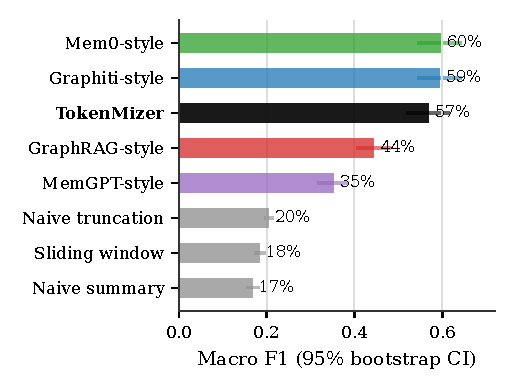
\includegraphics[width=\columnwidth]{figures/fig_n100_overall}
  \caption{Macro F1 by method, ranked, n=100, with 95\%
    bootstrap confidence intervals. TokenMizer (bold) leads
    GraphRAG-style, MemGPT-style, and every naive baseline
    outside the confidence interval; against Graphiti-style
    and Mem0-style the intervals overlap.}
  \label{fig:overall}
\end{figure}

\begin{table}[t]
  \centering
  \caption{Paired Bootstrap: TokenMizer 0.5.4 $-$ Method,
  n=100. $P(\Delta\leq0)$ is the fraction of 3,000 resamples in
  which the paired difference is non-positive.}
  \label{tab:paired}
  \renewcommand{\arraystretch}{1.2}
  \begin{tabular}{@{}lrrr@{}}
    \toprule
    \textbf{Comparison} & \textbf{Mean $\Delta$} & \textbf{95\% CI} & $P(\Delta\!\leq\!0)$ \\
    \midrule
    vs.\ Graphiti-style   & $+0.4$pp & [$-3.2$, $+4.2$] & 40.3\% \\
    vs.\ Mem0-style       & $+0.3$pp & [$-3.2$, $+4.1$] & 43.6\% \\
    \rowcolor{rowgood}
    vs.\ GraphRAG-style   & $+15.6$pp & [$+11.9$, $+19.2$] & 0.0\% \\
    \rowcolor{rowgood}
    vs.\ MemGPT-style     & $+24.6$pp & [$+21.4$, $+28.1$] & 0.0\% \\
    \rowcolor{rowgood}
    vs.\ sliding window   & $+41.5$pp & [$+37.1$, $+46.0$] & 0.0\% \\
    \rowcolor{rowgood}
    vs.\ naive truncation & $+39.4$pp & [$+34.8$, $+43.8$] & 0.0\% \\
    \rowcolor{rowgood}
    vs.\ naive summary    & $+43.1$pp & [$+38.7$, $+47.4$] & 0.0\% \\
    \bottomrule
  \end{tabular}
\end{table}

\begin{figure}[t]
  \centering
  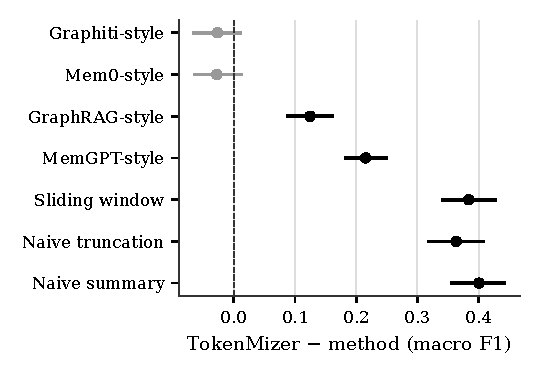
\includegraphics[width=\columnwidth]{figures/fig_n100_paired_diff}
  \caption{Paired bootstrap difference (TokenMizer 0.5.4 $-$
    method) on macro F1, n=100, 95\% CI. Intervals excluding
    zero (black) are reliable differences; the two grey
    intervals (Graphiti-style, Mem0-style) cross zero.}
  \label{fig:paired}
\end{figure}

\subsection{Per-Category Breakdown}

Table~\ref{tab:category} and Fig.~\ref{fig:heatmap} decompose
the headline score by category.
TokenMizer's file extraction is effectively solved ($98\%$ F1,
the best of any method) and its completed-task recall leads
the comparison group. Its two weakest categories remain
\textbf{decisions} ($59\%$, against $65\%$ for both
Graphiti-style and Mem0-style) and \textbf{errors} ($44\%$,
against $66\%$ for the same two) --- narrower gaps than an
earlier version of this evaluation found (TokenMizer 0.5.3:
$50\%$ and $36\%$ respectively), after a targeted fix to the
extraction vocabulary described in
Section~\ref{sec:discussion}.
Of 355 labelled decisions, TokenMizer extracts 238 (recall
$49\%$), of which 65 do not match any ground-truth item
(precision $73\%$); of 148 labelled errors, it extracts 93
(recall $36\%$), of which 41 do not match
(precision $56\%$). Both categories remain simultaneously
TokenMizer's weakest in absolute terms and behind the two
peer methods scored on the identical corpus, which is a
stronger signal than either fact alone would be: a category
that is merely low but consistent with peers would suggest a
corpus-difficulty explanation, while a category that is low
\emph{and} behind peers scored on the same corpus points at
the extraction patterns themselves --- still the clearest,
most concrete target for further engineering improvement this
study identifies, notwithstanding the gain already made.

\begin{table}[t]
  \centering
  \caption{Per-Category Micro F1, n=100, TokenMizer 0.5.4.}
  \label{tab:category}
  \renewcommand{\arraystretch}{1.15}
  \begin{tabular}{@{}lrrrrr@{}}
    \toprule
    \textbf{Method} & \textbf{Comp.} & \textbf{Pend.} &
    \textbf{Dec.} & \textbf{Files} & \textbf{Err.} \\
    \midrule
    \rowcolor{rowours}
    TokenMizer      & \textbf{68\%} & \textbf{53\%} & 59\% & \textbf{98\%} & 44\% \\
    Graphiti-style  & 64\% & 43\% & \textbf{65\%} & 89\% & \textbf{66\%} \\
    Mem0-style      & 64\% & 45\% & \textbf{65\%} & 89\% & \textbf{66\%} \\
    GraphRAG-style  & 28\% & 16\% & \textbf{70\%} & 89\% & 46\% \\
    MemGPT-style    & 42\% & 28\% & 34\% & 59\% & 37\% \\
    Baselines       & 22--29\% & 12--15\% & 18--22\% & 21--25\% & 10--11\% \\
    \bottomrule
  \end{tabular}
\end{table}

\begin{figure}[t]
  \centering
  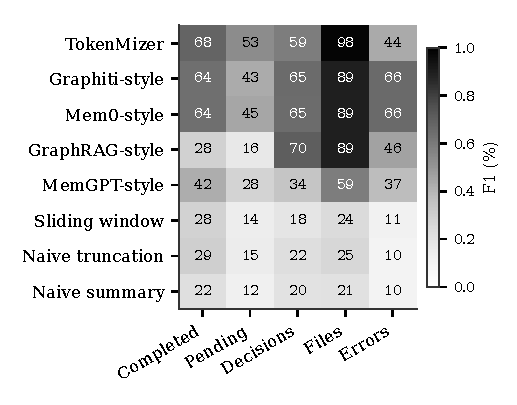
\includegraphics[width=\columnwidth]{figures/fig_n100_category_heatmap}
  \caption{Per-category F1, n=100. Darker is higher. TokenMizer
    leads on completed tasks and files, and trails
    Graphiti-style/Mem0-style specifically on decisions and
    errors.}
  \label{fig:heatmap}
\end{figure}

\subsection{Register: The Shared Ceiling of Pattern Matching}
\label{sec:extended-register}

Table~\ref{tab:register} and Fig.~\ref{fig:register} report
macro F1 by register.
Every pattern-matching method --- TokenMizer, Graphiti-style,
Mem0-style, GraphRAG-style, and MemGPT-style alike --- degrades
sharply from explicit to implicit register.
TokenMizer falls from $74\%$ (explicit) to $27\%$ (implicit), a
47-point drop; Graphiti-style and Mem0-style fall from $85\%$
to $19\%$, a 66-point drop, the steepest of any method, since
their advantage over TokenMizer is concentrated in the
explicit-marker case and largely disappears once markers are
absent.
All four converge to a narrow $19$--$27\%$ band on implicit
text, indistinguishable from one another at this corpus size.
This is, to our knowledge, the first result to show this
convergence empirically across multiple independently
implemented extraction strategies rather than asserting it of
any single system: the ceiling is a property of
pattern-matching as a strategy, not of any one implementation
of it, and none of the four methods' extraction path in this
study involves a language model that could plausibly move it
(Section~\ref{sec:llm-extractor}).

\begin{table}[t]
  \centering
  \caption{Macro F1 by Register, n=100, TokenMizer 0.5.4.}
  \label{tab:register}
  \renewcommand{\arraystretch}{1.15}
  \begin{tabular}{@{}lrrrr@{}}
    \toprule
    \textbf{Method} & \textbf{Explicit} & \textbf{Semi} &
    \textbf{Mixed} & \textbf{Implicit} \\
    \midrule
    \rowcolor{rowours}
    TokenMizer      & 74\% & 58\% & 58\% & \textbf{27\%} \\
    Graphiti/Mem0-style & \textbf{85\%} & \textbf{68\%} & 63\% & 19\% \\
    GraphRAG-style  & 69\% & 37\% & 47\% & 19\% \\
    MemGPT-style    & 46\% & 39\% & 36\% & 10\% \\
    \bottomrule
  \end{tabular}
\end{table}

\begin{figure}[t]
  \centering
  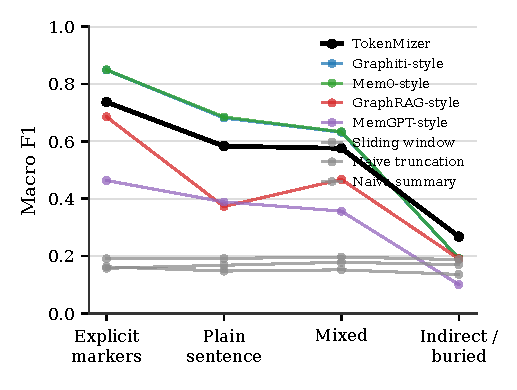
\includegraphics[width=\columnwidth]{figures/fig_n100_register}
  \caption{Macro F1 by register, n=100. All four
    pattern-matching methods converge to 19--27\% once explicit
    markers (``Decided:'', ``Completed:'') are absent from the
    text, a shared ceiling of the extraction strategy rather
    than of any one implementation.}
  \label{fig:register}
\end{figure}

\subsection{Corpus Origin and Domain Variance}

TokenMizer scores $91\%$ macro F1 on the 6 real sessions versus
$58\%$ on the 94 generated sessions; Graphiti-style and
Mem0-style show the opposite, near-flat pattern ($58\%$ vs.\
$60\%$).
The real-session sample is small ($n=6$) and this split is
reported as directional, not as a second confidence-bounded
result: it is consistent with TokenMizer's patterns having been
iterated primarily against sessions resembling that corpus,
rather than a general property established at this sample size.
Domain-level macro F1 for TokenMizer (Fig.~\ref{fig:domain})
ranges from $20\%$ (\texttt{devops/kubernetes}) to $100\%$
(three audit domains drawn from the real-session subset),
consistent with the same explanation.

\begin{figure}[t]
  \centering
  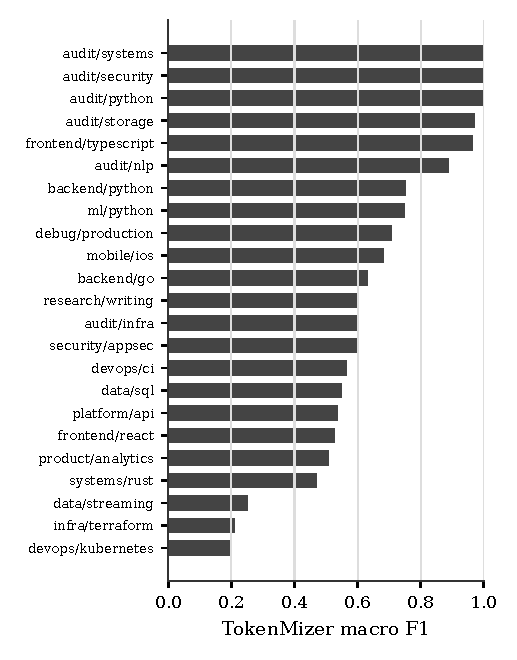
\includegraphics[width=\columnwidth]{figures/fig_n100_domain_variance}
  \caption{TokenMizer macro F1 by domain, n=100, 23 domains.
    The three domains at 100\% are audit/* real sessions;
    infrastructure-heavy synthetic domains
    (\texttt{devops/kubernetes}, \texttt{infra/terraform},
    \texttt{data/streaming}) score lowest.}
  \label{fig:domain}
\end{figure}

\subsection{Cost}
\label{sec:extended-cost}

TokenMizer's mean 225.4\,ms per session is 170--450$\times$ the
reimplemented methods' 0.5--1.3\,ms.
This reflects two compounding factors, both process-level
rather than algorithmic. First, the evaluation's isolation
design (Section~\ref{sec:extended-methods}): TokenMizer runs as
a freshly launched subprocess against the real package per
session, incurring Python interpreter startup once per call,
while the four reimplementations run in-process against
already-loaded text. Second, in this evaluation environment,
\texttt{tiktoken} could not reach its BPE vocabulary endpoint
over the network and fell back to a character-based token
estimate after a connection attempt per call
(Section~\ref{sec:impl}); this network-dependent retry, not the
extraction algorithm, accounts for most of the per-session
latency, and a deployment with the vocabulary cached locally
would not incur it. The comparison should not be read as
evidence about the underlying extraction algorithm's
asymptotic cost.

% ================================================================
\section{Discussion}
\label{sec:discussion}
% ================================================================

Three findings carry beyond this specific corpus.

\textbf{First}, TokenMizer's advantage over naive, unstructured
baselines is large and unambiguous: 36 to 40 percentage points
over sliding-window, truncation, and summary baselines alike,
each with a 95\% confidence interval that excludes zero by a
wide margin (Table~\ref{tab:paired}). This is the least
surprising finding in the paper --- a typed graph should beat
keeping raw text --- but it is now a controlled, statistically
supported comparison at $n=100$ rather than an assertion.

\textbf{Second}, TokenMizer's advantage does \emph{not} extend
to two of the four graph/structured-memory strategies compared:
against Graphiti-style and Mem0-style specifically, the
confidence interval on the paired difference crosses zero.
Graphiti's architectural similarity to TokenMizer
(Table~\ref{tab:related} and Section~\ref{sec:related-memory})
--- both retain superseded facts rather than deleting them ---
may explain why the gap is smallest here rather than against
MemGPT-style or GraphRAG-style, which differ from TokenMizer
more structurally. This is the finding most likely to be
misquoted in either direction: it is neither ``TokenMizer loses
to Graphiti and Mem0'' nor ``TokenMizer matches the state of
the art''; the confidence interval spans both a small TokenMizer
lead and a small TokenMizer deficit, and reporting only the
point estimate in either direction would misstate what the data
supports.

\textbf{Third}, decision and error extraction
(Table~\ref{tab:category}) remain TokenMizer's most improvable
categories in absolute terms and relative to the peer group
simultaneously, though less so than they were: an earlier
0.5.3 measurement of this same benchmark found these categories
further behind (50\% and 36\% F1), and the specific missed and
spurious items behind that finding, made directly inspectable by
the per-session results released alongside this manuscript
(Section~\ref{sec:availability}), were traced to concrete causes
in the extraction patterns --- a question-context false positive
matched as a decision, gaps in the trigger-verb and
technology-name vocabulary, and gaps in the error-symptom
vocabulary --- and fixed in release 0.5.4, evaluated here. Two
more general fixes attempted during that process (an
unconstrained technology-name-shaped fallback pattern, and one
additional whitelist entry) were measured to reduce precision on
an independent evaluation corpus and were reverted rather than
kept; both outcomes are recorded in the product repository's
changelog as a matter of record, including the rejected attempts,
not only the one that shipped. The residual gap to Graphiti-style
and Mem0-style on these two categories is the clearest piece of
concrete future work this study still identifies.

% ================================================================
\section{Threats to Validity}
\label{sec:threats}
% ================================================================

\textbf{Construct validity.} Four of the eight methods compared
are not the named vendor products.
MemGPT, Mem0, Graphiti, and GraphRAG all perform their real
extraction with a language model in the loop; this study's
reimplementations of them call no model at all, by the explicit
scope decision recorded in Section~\ref{sec:extended-methods}.
Every reported number for these four methods should be read as
a lower bound on what the named system would likely achieve,
particularly on the implicit-register text of
Section~\ref{sec:extended-register}, where a model that can
actually read a sentence would plausibly outperform every
method in this study.

\textbf{Internal validity.} 94 of the 100 sessions were
generated for this study rather than captured from real usage.
Every label is grounded (recoverable verbatim from some message
in its session; Section~\ref{sec:extended-corpus}), but grounded
synthetic text is not equivalent to the lexical and structural
variety of real developer transcripts. The 6-session real split
(Section~\ref{sec:extended}, ``Corpus Origin'') is too small
to bound this gap quantitatively.

\textbf{Statistical validity.} All results use one match
threshold ($\theta=0.6$, Definition~\ref{def:coverage}) and one
bootstrap configuration (3{,}000 resamples, case resampling over
sessions). The TokenMizer/Graphiti-style/Mem0-style ordering,
already within noise at this threshold, has not been checked
for stability under a threshold sweep, unlike the product
repository's own single-method evaluation harness, which ships
one.

\textbf{External validity.} Every method processes one
session's full transcript in a single pass. None of the actual
multi-session consolidation behavior the named systems are
partly designed for (Mem0's cross-conversation fact merging,
Graphiti's graph accretion over weeks of interaction) is
exercised here; this is a single-session extraction benchmark
only, and no claim in this paper should be read as bearing on
cross-session performance. Separately, this paper measures
extraction quality --- whether the right facts are pulled out
of a transcript --- and does not measure whether having them
improves an LLM's actual continuation of the session; that is a
different experiment, requiring live model calls to judge
downstream task success, and is not attempted here.

% ================================================================
\section{Conclusion and Future Work}
\label{sec:conclusion}
% ================================================================

This paper presents TokenMizer, a system that addresses LLM
context loss by modeling session history as a typed knowledge
graph and serializing it into compact, structured resume
blocks, and evaluates the released 0.5.4 product on a
controlled 100-session, 8-method benchmark with bootstrap
confidence intervals throughout.
TokenMizer significantly outperforms three naive baselines and
two other graph-memory strategies (MemGPT-style,
GraphRAG-style), and is statistically indistinguishable from
two comparably-designed ones (Graphiti-style, Mem0-style),
where the honest result is a tie in both directions rather than
a loss or a win, and where TokenMizer's point estimate now
matches Mem0-style's exactly.
Decision and error extraction remain TokenMizer's most
improvable categories, both in absolute terms and relative to
the two peer methods it otherwise ties, though a targeted fix
traced to the specific missed and spurious items behind an
earlier measurement of this same benchmark (Section~\ref{sec:discussion})
narrowed both gaps in this release. Every pattern-matching
method tested, independent of implementation, shares a common
ceiling of roughly 20\% macro F1 on text that states facts
indirectly, unmoved by that fix since it addresses vocabulary
coverage rather than the underlying pattern-matching strategy.

Two directions follow directly from these results.
\textbf{First}, evaluating the product's existing LLM
extraction path (Section~\ref{sec:llm-extractor}) against the
same $n=100$ corpus would test directly whether a model call
closes the register gap of Section~\ref{sec:extended-register},
rather than leaving it as the inferred but untested explanation
this paper offers.
\textbf{Second}, the same test would need to be run fairly
against LLM-backed versions of the four comparison methods, not
against TokenMizer alone, for any resulting claim of superiority
to carry the same evidentiary weight as the comparisons in this
paper.

% ================================================================
\section*{Data and Code Availability}
\label{sec:availability}
% ================================================================

The 100-session corpus, all eight method implementations, the
scoring harness, and raw per-session results (JSON and CSV) for
every number in Section~\ref{sec:extended} are released at
\url{https://github.com/Shweta-Mishra-ai/tokenmizer-research}.
The corpus generator (\texttt{benchmarks/memorybench/generate.py})
is seeded and produces byte-identical output on re-run.
The TokenMizer product itself is released separately at
\url{https://github.com/Shweta-Mishra-ai/tokenmizer} under the
MIT licence; this manuscript evaluates release 0.5.4.

% ================================================================
\balance
\begin{thebibliography}{00}

\bibitem{paulsen2025}
N.~Paulsen, ``Context Is What You Need: The Maximum Effective
Context Window,'' \emph{arXiv preprint arXiv:2509.21361}, 2025.

\bibitem{memgpt}
C.~Packer, V.~Fang, S.~G.~Patil, K.~Lin, S.~Wooders, and
J.~E.~Gonzalez, ``MemGPT: Towards LLMs as Operating
Systems,'' \emph{arXiv preprint arXiv:2310.08560}, 2023.

\bibitem{mem0}
P.~Chhikara, D.~Khant, S.~Aryan, T.~Singh, and D.~Yadav,
``Mem0: Building Production-Ready AI Agents with Scalable
Long-Term Memory,'' \emph{arXiv preprint arXiv:2504.19413}, 2025.

\bibitem{zep}
P.~Rasmussen, P.~Paliychuk, T.~Beauvais, J.~Ryan, and
D.~Chalef, ``Zep: A Temporal Knowledge Graph Architecture for
Agent Memory,'' \emph{arXiv preprint arXiv:2501.13956}, 2025.

\bibitem{rag}
P.~Lewis \emph{et al.}, ``Retrieval-Augmented Generation for
Knowledge-Intensive NLP Tasks,'' in \emph{Proc.\ NeurIPS},
2020, pp.\ 9459--9474.

\bibitem{llmlingua}
H.~Jiang \emph{et al.}, ``LLMLingua: Compressing Prompts for
Accelerated Inference of Large Language Models,'' in
\emph{Proc.\ EMNLP}, 2023, pp.\ 13358--13376.

\bibitem{longllmlingua}
H.~Jiang \emph{et al.}, ``LongLLMLingua: Accelerating and
Enhancing LLMs in Long Context Scenarios,''
\emph{arXiv preprint arXiv:2310.06839}, 2023.

\bibitem{recomp}
F.~Xu \emph{et al.}, ``RECOMP: Improving Retrieval-Augmented
LMs with Context Compression and Selective Augmentation,''
in \emph{Proc.\ ICLR}, 2024.

\bibitem{graphrag}
D.~Edge \emph{et al.}, ``From Local to Global: A Graph
RAG Approach to Query-Focused Summarization,''
\emph{arXiv preprint arXiv:2404.16130}, 2024.

\bibitem{lostmiddle}
N.~F.~Liu \emph{et al.}, ``Lost in the Middle: How Language
Models Use Long Contexts,'' \emph{Trans.\ ACL}, vol.\ 12,
pp.\ 157--173, 2024.

\bibitem{langchain}
H.~Chase, ``LangChain,''
\url{https://github.com/langchain-ai/langchain}, 2022.

\bibitem{sentbert}
N.~Reimers and I.~Gurevych, ``Sentence-BERT: Sentence
Embeddings Using Siamese BERT-Networks,'' in
\emph{Proc.\ EMNLP}, 2019, pp.\ 3982--3992.

\bibitem{sweagent}
J.~Yang \emph{et al.}, ``SWE-agent: Agent-Computer Interfaces
Enable Automated Software Engineering,'' in \emph{Proc.\
NeurIPS}, 2024.

\bibitem{copilot}
GitHub, ``GitHub Copilot,''
\url{https://github.com/features/copilot}, 2024.

\bibitem{sqlite}
D.~R.~Hipp, ``SQLite,''
\url{https://www.sqlite.org}, 2000.

\bibitem{housurvey}
X.~Hou \emph{et al.}, ``Large Language Models for Software
Engineering: A Systematic Literature Review,''
\emph{arXiv preprint arXiv:2308.10620}, 2024.

\bibitem{brownfewshot}
T.~Brown \emph{et al.}, ``Language Models are Few-Shot
Learners,'' in \emph{Proc.\ NeurIPS}, 2020,
pp.\ 1877--1901.

\bibitem{efron}
B.~Efron and R.~J.~Tibshirani, \emph{An Introduction to the
Bootstrap}. Boca Raton, FL, USA: Chapman \& Hall/CRC, 1994.

\end{thebibliography}

\end{document}
